%-*-latex-*-
\sectionthree{Increase-key and decrease-key}
\begin{python0}
from solutions import *; clear()
\end{python0}

So suppose I already have a priority queue (as a heap):

\begin{center}
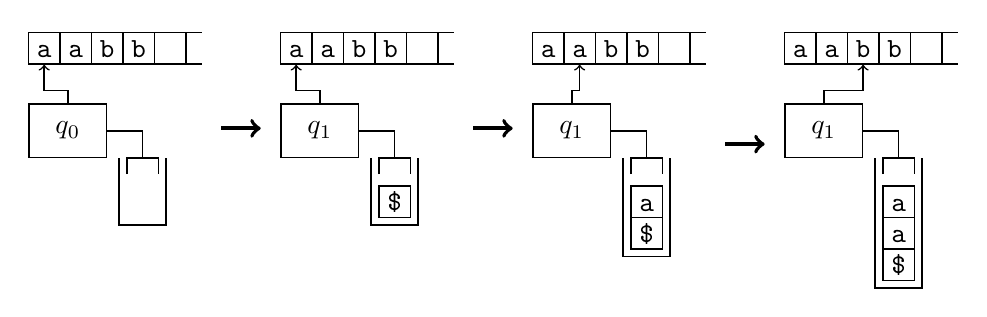
\begin{tikzpicture}

\draw (0.2, 0.2)
  node[draw, line width=0.02cm, , color=black,
       rounded corners=0cm, inner sep=0cm] {

\begin{minipage}[t][0.4cm]{0.4cm}
\mbox{}

\end{minipage}

};\draw (0.2, 0.2) node[color=black] {{\vphantom{aabb\SPACE}\texttt{a}}};
\draw (0.6000000000000001, 0.2)
  node[draw, line width=0.02cm, , color=black,
       rounded corners=0cm, inner sep=0cm] {

\begin{minipage}[t][0.4cm]{0.4cm}
\mbox{}

\end{minipage}

};\draw (0.6000000000000001, 0.2) node[color=black] {{\vphantom{aabb\SPACE}\texttt{a}}};
\draw (1.0, 0.2)
  node[draw, line width=0.02cm, , color=black,
       rounded corners=0cm, inner sep=0cm] {

\begin{minipage}[t][0.4cm]{0.4cm}
\mbox{}

\end{minipage}

};\draw (1.0, 0.2) node[color=black] {{\vphantom{aabb\SPACE}\texttt{b}}};
\draw (1.4000000000000001, 0.2)
  node[draw, line width=0.02cm, , color=black,
       rounded corners=0cm, inner sep=0cm] {

\begin{minipage}[t][0.4cm]{0.4cm}
\mbox{}

\end{minipage}

};\draw (1.4000000000000001, 0.2) node[color=black] {{\vphantom{aabb\SPACE}\texttt{b}}};
\draw (1.7999999999999998, 0.2)
  node[draw, line width=0.02cm, , color=black,
       rounded corners=0cm, inner sep=0cm] {

\begin{minipage}[t][0.4cm]{0.4cm}
\mbox{}

\end{minipage}

};\draw (1.7999999999999998, 0.2) node[color=black] {{\vphantom{aabb\SPACE}\texttt{\SPACE}}};\draw[line width=0.02cm,black] (2.0,0.4) to  (2.2,0.4);
\draw[line width=0.02cm,black] (2.0,0.0) to  (2.2,0.0);

\draw (0.5, -0.85)
  node[draw, line width=0.02cm, , color=black,
       rounded corners=0cm, inner sep=0cm] {

\begin{minipage}[t][0.68cm]{0.98cm}
\mbox{}

\end{minipage}

};\draw (0.5, -0.85) node[color=black] {$q_0$};\draw[line width=0.02cm,black,->] (0.5,-0.5) to  (0.5,-0.34) to  (0.2,-0.34) to  (0.2,-0.01);

\draw (1.45, -1.7499999999999998)
  node[draw=none, line width=0cm, , color=black,
       rounded corners=0cm, inner sep=0cm] {

\begin{minipage}[t][0.4cm]{0.4cm}
\mbox{}

\end{minipage}

};\draw[line width=0.02cm,black] (1.15,-1.2) to  (1.15,-2.05) to  (1.75,-2.05) to  (1.75,-1.2);
\draw[line width=0.02cm,black] (1,-0.85) to  (1.45,-0.85) to  (1.45,-1.2);
\draw[line width=0.02cm,black] (1.25,-1.4) to  (1.25,-1.2) to  (1.65,-1.2) to  (1.65,-1.4);
\draw[line width=0.05cm,black,->] (2.45,-0.82) to  (2.95,-0.82);

\draw (3.4000000000000004, 0.2)
  node[draw, line width=0.02cm, , color=black,
       rounded corners=0cm, inner sep=0cm] {

\begin{minipage}[t][0.4cm]{0.4cm}
\mbox{}

\end{minipage}

};\draw (3.4000000000000004, 0.2) node[color=black] {{\vphantom{\$aabb\SPACE}\texttt{a}}};
\draw (3.8, 0.2)
  node[draw, line width=0.02cm, , color=black,
       rounded corners=0cm, inner sep=0cm] {

\begin{minipage}[t][0.4cm]{0.4cm}
\mbox{}

\end{minipage}

};\draw (3.8, 0.2) node[color=black] {{\vphantom{\$aabb\SPACE}\texttt{a}}};
\draw (4.2, 0.2)
  node[draw, line width=0.02cm, , color=black,
       rounded corners=0cm, inner sep=0cm] {

\begin{minipage}[t][0.4cm]{0.4cm}
\mbox{}

\end{minipage}

};\draw (4.2, 0.2) node[color=black] {{\vphantom{\$aabb\SPACE}\texttt{b}}};
\draw (4.6000000000000005, 0.2)
  node[draw, line width=0.02cm, , color=black,
       rounded corners=0cm, inner sep=0cm] {

\begin{minipage}[t][0.4cm]{0.4cm}
\mbox{}

\end{minipage}

};\draw (4.6000000000000005, 0.2) node[color=black] {{\vphantom{\$aabb\SPACE}\texttt{b}}};
\draw (5.000000000000001, 0.2)
  node[draw, line width=0.02cm, , color=black,
       rounded corners=0cm, inner sep=0cm] {

\begin{minipage}[t][0.4cm]{0.4cm}
\mbox{}

\end{minipage}

};\draw (5.000000000000001, 0.2) node[color=black] {{\vphantom{\$aabb\SPACE}\texttt{\SPACE}}};\draw[line width=0.02cm,black] (5.200000000000001,0.4) to  (5.4,0.4);
\draw[line width=0.02cm,black] (5.200000000000001,0.0) to  (5.4,0.0);

\draw (3.7, -0.85)
  node[draw, line width=0.02cm, , color=black,
       rounded corners=0cm, inner sep=0cm] {

\begin{minipage}[t][0.68cm]{0.98cm}
\mbox{}

\end{minipage}

};\draw (3.7, -0.85) node[color=black] {$q_1$};\draw[line width=0.02cm,black,->] (3.7,-0.5) to  (3.7,-0.34) to  (3.4,-0.34) to  (3.4,-0.01);

\draw (4.65, -1.7499999999999998)
  node[draw, line width=0.02cm, , color=black,
       rounded corners=0cm, inner sep=0cm] {

\begin{minipage}[t][0.4cm]{0.4cm}
\mbox{}

\end{minipage}

};\draw (4.65, -1.7499999999999998) node[color=black] {{\vphantom{\$aabb\SPACE}\texttt{\$}}};\draw[line width=0.02cm,black] (4.35,-1.2) to  (4.35,-2.05) to  (4.95,-2.05) to  (4.95,-1.2);
\draw[line width=0.02cm,black] (4.2,-0.85) to  (4.65,-0.85) to  (4.65,-1.2);
\draw[line width=0.02cm,black] (4.45,-1.4) to  (4.45,-1.2) to  (4.85,-1.2) to  (4.85,-1.4);
\draw[line width=0.05cm,black,->] (5.65,-0.82) to  (6.15,-0.82);

\draw (6.600000000000001, 0.2)
  node[draw, line width=0.02cm, , color=black,
       rounded corners=0cm, inner sep=0cm] {

\begin{minipage}[t][0.4cm]{0.4cm}
\mbox{}

\end{minipage}

};\draw (6.600000000000001, 0.2) node[color=black] {{\vphantom{a\$aabb\SPACE}\texttt{a}}};
\draw (7.000000000000002, 0.2)
  node[draw, line width=0.02cm, , color=black,
       rounded corners=0cm, inner sep=0cm] {

\begin{minipage}[t][0.4cm]{0.4cm}
\mbox{}

\end{minipage}

};\draw (7.000000000000002, 0.2) node[color=black] {{\vphantom{a\$aabb\SPACE}\texttt{a}}};
\draw (7.400000000000002, 0.2)
  node[draw, line width=0.02cm, , color=black,
       rounded corners=0cm, inner sep=0cm] {

\begin{minipage}[t][0.4cm]{0.4cm}
\mbox{}

\end{minipage}

};\draw (7.400000000000002, 0.2) node[color=black] {{\vphantom{a\$aabb\SPACE}\texttt{b}}};
\draw (7.8000000000000025, 0.2)
  node[draw, line width=0.02cm, , color=black,
       rounded corners=0cm, inner sep=0cm] {

\begin{minipage}[t][0.4cm]{0.4cm}
\mbox{}

\end{minipage}

};\draw (7.8000000000000025, 0.2) node[color=black] {{\vphantom{a\$aabb\SPACE}\texttt{b}}};
\draw (8.200000000000003, 0.2)
  node[draw, line width=0.02cm, , color=black,
       rounded corners=0cm, inner sep=0cm] {

\begin{minipage}[t][0.4cm]{0.4cm}
\mbox{}

\end{minipage}

};\draw (8.200000000000003, 0.2) node[color=black] {{\vphantom{a\$aabb\SPACE}\texttt{\SPACE}}};\draw[line width=0.02cm,black] (8.400000000000002,0.4) to  (8.600000000000001,0.4);
\draw[line width=0.02cm,black] (8.400000000000002,0.0) to  (8.600000000000001,0.0);

\draw (6.900000000000001, -0.85)
  node[draw, line width=0.02cm, , color=black,
       rounded corners=0cm, inner sep=0cm] {

\begin{minipage}[t][0.68cm]{0.98cm}
\mbox{}

\end{minipage}

};\draw (6.900000000000001, -0.85) node[color=black] {$q_1$};\draw[line width=0.02cm,black,->] (6.9,-0.5) to  (6.9,-0.34) to  (7.0,-0.34) to  (7.0,-0.01);

\draw (7.850000000000001, -1.7499999999999998)
  node[draw, line width=0.02cm, , color=black,
       rounded corners=0cm, inner sep=0cm] {

\begin{minipage}[t][0.4cm]{0.4cm}
\mbox{}

\end{minipage}

};\draw (7.850000000000001, -1.7499999999999998) node[color=black] {{\vphantom{a\$aabb\SPACE}\texttt{a}}};
\draw (7.850000000000001, -2.1499999999999995)
  node[draw, line width=0.02cm, , color=black,
       rounded corners=0cm, inner sep=0cm] {

\begin{minipage}[t][0.4cm]{0.4cm}
\mbox{}

\end{minipage}

};\draw (7.850000000000001, -2.1499999999999995) node[color=black] {{\vphantom{a\$aabb\SPACE}\texttt{\$}}};\draw[line width=0.02cm,black] (7.55,-1.2) to  (7.55,-2.45) to  (8.15,-2.45) to  (8.15,-1.2);
\draw[line width=0.02cm,black] (7.4,-0.85) to  (7.85,-0.85) to  (7.85,-1.2);
\draw[line width=0.02cm,black] (7.65,-1.4) to  (7.65,-1.2) to  (8.05,-1.2) to  (8.05,-1.4);
\draw[line width=0.05cm,black,->] (8.85,-1.02) to  (9.35,-1.02);

\draw (9.8, 0.2)
  node[draw, line width=0.02cm, , color=black,
       rounded corners=0cm, inner sep=0cm] {

\begin{minipage}[t][0.4cm]{0.4cm}
\mbox{}

\end{minipage}

};\draw (9.8, 0.2) node[color=black] {{\vphantom{aa\$aabb\SPACE}\texttt{a}}};
\draw (10.200000000000003, 0.2)
  node[draw, line width=0.02cm, , color=black,
       rounded corners=0cm, inner sep=0cm] {

\begin{minipage}[t][0.4cm]{0.4cm}
\mbox{}

\end{minipage}

};\draw (10.200000000000003, 0.2) node[color=black] {{\vphantom{aa\$aabb\SPACE}\texttt{a}}};
\draw (10.600000000000001, 0.2)
  node[draw, line width=0.02cm, , color=black,
       rounded corners=0cm, inner sep=0cm] {

\begin{minipage}[t][0.4cm]{0.4cm}
\mbox{}

\end{minipage}

};\draw (10.600000000000001, 0.2) node[color=black] {{\vphantom{aa\$aabb\SPACE}\texttt{b}}};
\draw (11.000000000000004, 0.2)
  node[draw, line width=0.02cm, , color=black,
       rounded corners=0cm, inner sep=0cm] {

\begin{minipage}[t][0.4cm]{0.4cm}
\mbox{}

\end{minipage}

};\draw (11.000000000000004, 0.2) node[color=black] {{\vphantom{aa\$aabb\SPACE}\texttt{b}}};
\draw (11.400000000000002, 0.2)
  node[draw, line width=0.02cm, , color=black,
       rounded corners=0cm, inner sep=0cm] {

\begin{minipage}[t][0.4cm]{0.4cm}
\mbox{}

\end{minipage}

};\draw (11.400000000000002, 0.2) node[color=black] {{\vphantom{aa\$aabb\SPACE}\texttt{\SPACE}}};\draw[line width=0.02cm,black] (11.600000000000003,0.4) to  (11.800000000000002,0.4);
\draw[line width=0.02cm,black] (11.600000000000003,0.0) to  (11.800000000000002,0.0);

\draw (10.100000000000001, -0.85)
  node[draw, line width=0.02cm, , color=black,
       rounded corners=0cm, inner sep=0cm] {

\begin{minipage}[t][0.68cm]{0.98cm}
\mbox{}

\end{minipage}

};\draw (10.100000000000001, -0.85) node[color=black] {$q_1$};\draw[line width=0.02cm,black,->] (10.1,-0.5) to  (10.1,-0.34) to  (10.6,-0.34) to  (10.6,-0.01);

\draw (11.05, -1.7499999999999998)
  node[draw, line width=0.02cm, , color=black,
       rounded corners=0cm, inner sep=0cm] {

\begin{minipage}[t][0.4cm]{0.4cm}
\mbox{}

\end{minipage}

};\draw (11.05, -1.7499999999999998) node[color=black] {{\vphantom{aa\$aabb\SPACE}\texttt{a}}};
\draw (11.05, -2.1499999999999995)
  node[draw, line width=0.02cm, , color=black,
       rounded corners=0cm, inner sep=0cm] {

\begin{minipage}[t][0.4cm]{0.4cm}
\mbox{}

\end{minipage}

};\draw (11.05, -2.1499999999999995) node[color=black] {{\vphantom{aa\$aabb\SPACE}\texttt{a}}};
\draw (11.05, -2.55)
  node[draw, line width=0.02cm, , color=black,
       rounded corners=0cm, inner sep=0cm] {

\begin{minipage}[t][0.4cm]{0.4cm}
\mbox{}

\end{minipage}

};\draw (11.05, -2.55) node[color=black] {{\vphantom{aa\$aabb\SPACE}\texttt{\$}}};\draw[line width=0.02cm,black] (10.75,-1.2) to  (10.75,-2.85) to  (11.35,-2.85) to  (11.35,-1.2);
\draw[line width=0.02cm,black] (10.6,-0.85) to  (11.05,-0.85) to  (11.05,-1.2);
\draw[line width=0.02cm,black] (10.85,-1.4) to  (10.85,-1.2) to  (11.25,-1.2) to  (11.25,-1.4);
\end{tikzpicture}

\end{center}




Suppose \texttt{1} is increased to \texttt{12}:

\begin{center}
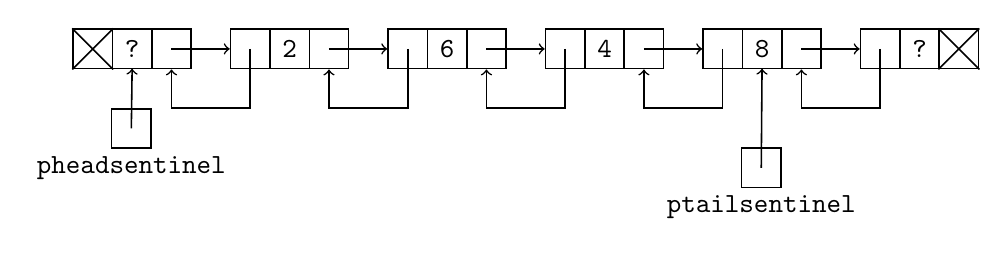
\begin{tikzpicture}

\draw (0.25, 0.25)
  node[draw, line width=0.02cm, , color=black,
       rounded corners=0cm, inner sep=0cm] {

\begin{minipage}[t][0.5cm]{0.5cm}
\mbox{}

\end{minipage}

};\draw (0.25, 0.25) node[color=black] {{\texttt{}}};
\draw (0.75, 0.25)
  node[draw, line width=0.02cm, , color=black,
       rounded corners=0cm, inner sep=0cm] {

\begin{minipage}[t][0.5cm]{0.5cm}
\mbox{}

\end{minipage}

};\draw (0.75, 0.25) node[color=black] {{\texttt{?}}};
\draw (1.25, 0.25)
  node[draw, line width=0.02cm, , color=black,
       rounded corners=0cm, inner sep=0cm] {

\begin{minipage}[t][0.5cm]{0.5cm}
\mbox{}

\end{minipage}

};\draw (1.25, 0.25) node[color=black] {{\texttt{}}};
\draw (2.25, 0.25)
  node[draw, line width=0.02cm, , color=black,
       rounded corners=0cm, inner sep=0cm] {

\begin{minipage}[t][0.5cm]{0.5cm}
\mbox{}

\end{minipage}

};\draw (2.25, 0.25) node[color=black] {{\texttt{}}};
\draw (2.75, 0.25)
  node[draw, line width=0.02cm, , color=black,
       rounded corners=0cm, inner sep=0cm] {

\begin{minipage}[t][0.5cm]{0.5cm}
\mbox{}

\end{minipage}

};\draw (2.75, 0.25) node[color=black] {{\texttt{2}}};
\draw (3.25, 0.25)
  node[draw, line width=0.02cm, , color=black,
       rounded corners=0cm, inner sep=0cm] {

\begin{minipage}[t][0.5cm]{0.5cm}
\mbox{}

\end{minipage}

};\draw (3.25, 0.25) node[color=black] {{\texttt{}}};
\draw (4.25, 0.25)
  node[draw, line width=0.02cm, , color=black,
       rounded corners=0cm, inner sep=0cm] {

\begin{minipage}[t][0.5cm]{0.5cm}
\mbox{}

\end{minipage}

};\draw (4.25, 0.25) node[color=black] {{\texttt{}}};
\draw (4.75, 0.25)
  node[draw, line width=0.02cm, , color=black,
       rounded corners=0cm, inner sep=0cm] {

\begin{minipage}[t][0.5cm]{0.5cm}
\mbox{}

\end{minipage}

};\draw (4.75, 0.25) node[color=black] {{\texttt{6}}};
\draw (5.25, 0.25)
  node[draw, line width=0.02cm, , color=black,
       rounded corners=0cm, inner sep=0cm] {

\begin{minipage}[t][0.5cm]{0.5cm}
\mbox{}

\end{minipage}

};\draw (5.25, 0.25) node[color=black] {{\texttt{}}};
\draw (6.25, 0.25)
  node[draw, line width=0.02cm, , color=black,
       rounded corners=0cm, inner sep=0cm] {

\begin{minipage}[t][0.5cm]{0.5cm}
\mbox{}

\end{minipage}

};\draw (6.25, 0.25) node[color=black] {{\texttt{}}};
\draw (6.75, 0.25)
  node[draw, line width=0.02cm, , color=black,
       rounded corners=0cm, inner sep=0cm] {

\begin{minipage}[t][0.5cm]{0.5cm}
\mbox{}

\end{minipage}

};\draw (6.75, 0.25) node[color=black] {{\texttt{4}}};
\draw (7.25, 0.25)
  node[draw, line width=0.02cm, , color=black,
       rounded corners=0cm, inner sep=0cm] {

\begin{minipage}[t][0.5cm]{0.5cm}
\mbox{}

\end{minipage}

};\draw (7.25, 0.25) node[color=black] {{\texttt{}}};
\draw (8.25, 0.25)
  node[draw, line width=0.02cm, , color=black,
       rounded corners=0cm, inner sep=0cm] {

\begin{minipage}[t][0.5cm]{0.5cm}
\mbox{}

\end{minipage}

};\draw (8.25, 0.25) node[color=black] {{\texttt{}}};
\draw (8.75, 0.25)
  node[draw, line width=0.02cm, , color=black,
       rounded corners=0cm, inner sep=0cm] {

\begin{minipage}[t][0.5cm]{0.5cm}
\mbox{}

\end{minipage}

};\draw (8.75, 0.25) node[color=black] {{\texttt{8}}};
\draw (9.25, 0.25)
  node[draw, line width=0.02cm, , color=black,
       rounded corners=0cm, inner sep=0cm] {

\begin{minipage}[t][0.5cm]{0.5cm}
\mbox{}

\end{minipage}

};\draw (9.25, 0.25) node[color=black] {{\texttt{}}};
\draw (10.25, 0.25)
  node[draw, line width=0.02cm, , color=black,
       rounded corners=0cm, inner sep=0cm] {

\begin{minipage}[t][0.5cm]{0.5cm}
\mbox{}

\end{minipage}

};\draw (10.25, 0.25) node[color=black] {{\texttt{}}};
\draw (10.75, 0.25)
  node[draw, line width=0.02cm, , color=black,
       rounded corners=0cm, inner sep=0cm] {

\begin{minipage}[t][0.5cm]{0.5cm}
\mbox{}

\end{minipage}

};\draw (10.75, 0.25) node[color=black] {{\texttt{?}}};
\draw (11.25, 0.25)
  node[draw, line width=0.02cm, , color=black,
       rounded corners=0cm, inner sep=0cm] {

\begin{minipage}[t][0.5cm]{0.5cm}
\mbox{}

\end{minipage}

};\draw (11.25, 0.25) node[color=black] {{\texttt{}}};\draw[line width=0.02cm,black,->] (1.25,0.25) to  (1.99,0.25);
\draw[line width=0.02cm,black,->] (3.25,0.25) to  (3.99,0.25);
\draw[line width=0.02cm,black,->] (2.25,0.25) to  (2.25,-0.5) to  (1.25,-0.5) to  (1.25,-0.01);
\draw[line width=0.02cm,black,->] (5.25,0.25) to  (5.99,0.25);
\draw[line width=0.02cm,black,->] (4.25,0.25) to  (4.25,-0.5) to  (3.25,-0.5) to  (3.25,-0.01);
\draw[line width=0.02cm,black,->] (7.25,0.25) to  (7.99,0.25);
\draw[line width=0.02cm,black,->] (6.25,0.25) to  (6.25,-0.5) to  (5.25,-0.5) to  (5.25,-0.01);
\draw[line width=0.02cm,black,->] (9.25,0.25) to  (9.99,0.25);
\draw[line width=0.02cm,black,->] (8.25,0.25) to  (8.25,-0.5) to  (7.25,-0.5) to  (7.25,-0.01);
\draw[line width=0.02cm,black,->] (10.25,0.25) to  (10.25,-0.5) to  (9.25,-0.5) to  (9.25,-0.01);
\draw[line width=0.02cm,black] (-0.01,0.51) to  (0.51,-0.01);
\draw[line width=0.02cm,black] (0.51,0.51) to  (-0.01,-0.01);
\draw[line width=0.02cm,black] (10.99,0.51) to  (11.51,-0.01);
\draw[line width=0.02cm,black] (11.51,0.51) to  (10.99,-0.01);

\draw (0.74, -0.76)
  node[draw, line width=0.02cm, , color=black,
       rounded corners=0cm, inner sep=0cm] {

\begin{minipage}[t][0.5cm]{0.5cm}
\mbox{}

\end{minipage}

};\draw (0.74, -0.76) node[color=black] {{\texttt{}}};
\draw (0.74, -1.26)
  node[draw, line width=0.02cm, , color=white,
       rounded corners=0cm, inner sep=0cm] {

\begin{minipage}[t][0.1cm]{0.1cm}
\mbox{}

\end{minipage}

};\draw (0.74, -1.26) node[color=black] {{\texttt{pheadsentinel}}};\draw[line width=0.02cm,black,->] (0.74,-0.76) to  (0.75,0);

\draw (8.74, -1.26)
  node[draw, line width=0.02cm, , color=black,
       rounded corners=0cm, inner sep=0cm] {

\begin{minipage}[t][0.5cm]{0.5cm}
\mbox{}

\end{minipage}

};\draw (8.74, -1.26) node[color=black] {{\texttt{}}};
\draw (8.74, -1.76)
  node[draw, line width=0.02cm, , color=white,
       rounded corners=0cm, inner sep=0cm] {

\begin{minipage}[t][0.1cm]{0.1cm}
\mbox{}

\end{minipage}

};\draw (8.74, -1.76) node[color=black] {{\texttt{ptailsentinel}}};\draw[line width=0.02cm,black,->] (8.74,-1.26) to  (8.75,0);
\end{tikzpicture}

\end{center}




I'm sure you can see very quickly that in order to make this back to
a maxheap, I need to heapify-up \texttt{12}.
In this case I need to swap 3 times to get this:

\begin{center}
\begin{tikzpicture}

\fill[white] (11.0, 0.0) circle (0.3);
\node [line width=0.03cm,black,minimum size=0.57cm,draw,circle] at (11.0,0.0)(A){};\draw (11.0, 0.0) node[color=black] {\texttt{20}};
\fill[white] (10.0, -0.7) circle (0.3);
\node [line width=0.03cm,black,minimum size=0.57cm,draw,circle] at (10.0,-0.7)(a){};\draw (10.0, -0.7) node[color=black] {\texttt{10}};
\fill[white] (8.0, -2.1) circle (0.3);
\node [line width=0.03cm,black,minimum size=0.57cm,draw,circle] at (8.0,-2.1)(e){};\draw (8.0, -2.1) node[color=black] {\texttt{-2}};
\fill[white] (7.0, -2.8) circle (0.3);
\node [line width=0.03cm,black,minimum size=0.57cm,draw,circle] at (7.0,-2.8)(k){};\draw (7.0, -2.8) node[color=black] {\texttt{-3}};
\fill[white] (9.0, -2.8) circle (0.3);
\node [line width=0.03cm,black,minimum size=0.57cm,draw,circle] at (9.0,-2.8)(l){};\draw (9.0, -2.8) node[color=black] {\texttt{-1}};
\fill[white] (11.0, -1.4) circle (0.3);
\node [line width=0.03cm,black,minimum size=0.57cm,draw,circle] at (11.0,-1.4)(p){};\draw (11.0, -1.4) node[color=black] {\texttt{15}};\draw[line width=0.03cm,black,->,>=triangle 60] (A) to  (a);
\draw[line width=0.03cm,black,->,>=triangle 60] (a) to  (p);
\draw[line width=0.03cm,black,->,>=triangle 60] (a) to  (e);
\draw[line width=0.03cm,black,->,>=triangle 60] (e) to  (k);
\draw[line width=0.03cm,black,->,>=triangle 60] (e) to  (l);
\end{tikzpicture}

\end{center}

\begin{center}
\begin{tikzpicture}

\fill[white] (11.0, 0.0) circle (0.3);
\node [line width=0.03cm,black,minimum size=0.57cm,draw,circle] at (11.0,0.0)(A){};\draw (11.0, 0.0) node[color=black] {\texttt{20}};
\fill[white] (10.0, -0.7) circle (0.3);
\node [line width=0.03cm,black,minimum size=0.57cm,draw,circle] at (10.0,-0.7)(a){};\draw (10.0, -0.7) node[color=black] {\texttt{10}};
\fill[white] (9.0, -1.4) circle (0.3);
\node [line width=0.03cm,black,minimum size=0.57cm,draw,circle] at (9.0,-1.4)(b){};\draw (9.0, -1.4) node[color=black] {\texttt{0}};
\fill[white] (8.0, -2.1) circle (0.3);
\node [line width=0.03cm,black,minimum size=0.57cm,draw,circle] at (8.0,-2.1)(e){};\draw (8.0, -2.1) node[color=black] {\texttt{-2}};
\fill[white] (7.0, -2.8) circle (0.3);
\node [line width=0.03cm,black,minimum size=0.57cm,draw,circle] at (7.0,-2.8)(k){};\draw (7.0, -2.8) node[color=black] {\texttt{-3}};
\fill[white] (9.0, -2.8) circle (0.3);
\node [line width=0.03cm,black,minimum size=0.57cm,draw,circle] at (9.0,-2.8)(l){};\draw (9.0, -2.8) node[color=black] {\texttt{-1}};
\fill[white] (11.0, -1.4) circle (0.3);
\node [line width=0.03cm,black,minimum size=0.57cm,draw,circle] at (11.0,-1.4)(p){};\draw (11.0, -1.4) node[color=black] {\texttt{15}};\draw[line width=0.03cm,black,->,>=triangle 60] (A) to  (a);
\draw[line width=0.03cm,black,->,>=triangle 60] (a) to  (p);
\draw[line width=0.03cm,black,->,>=triangle 60] (a) to  (b);
\draw[line width=0.03cm,black,->,>=triangle 60] (b) to  (e);
\draw[line width=0.03cm,black,->,>=triangle 60] (e) to  (k);
\draw[line width=0.03cm,black,->,>=triangle 60] (e) to  (l);
\end{tikzpicture}

\end{center}



\begin{console}
ALGORITHM: increase_key (for max heap)
INPUT: x - heap (using an array)
       n - length of heap in x
       i - index where key will increase
       k - new key value (k > x[i])

x[i] = k # originally x[i] < k
Perform heapify-up on x starting at index i.
\end{console}
So if the above represent processes with priorities, the low priority
process moves up, in fact to the top, so it will be the next process to
be executed.
The worse runtime of increase-key for max heap is
\[
O(\log n)
\]

Using the above tree

\begin{center}
\begin{tikzpicture}

\fill[white] (11.0, 0.0) circle (0.3);
\node [line width=0.03cm,black,minimum size=0.57cm,draw,circle] at (11.0,0.0)(A){};\draw (11.0, 0.0) node[color=black] {\texttt{20}};
\fill[white] (10.0, -0.7) circle (0.3);
\node [line width=0.03cm,black,minimum size=0.57cm,draw,circle] at (10.0,-0.7)(a){};\draw (10.0, -0.7) node[color=black] {\texttt{10}};
\fill[white] (9.0, -1.4) circle (0.3);
\node [line width=0.03cm,black,minimum size=0.57cm,draw,circle] at (9.0,-1.4)(b){};\draw (9.0, -1.4) node[color=black] {\texttt{0}};
\fill[white] (8.0, -2.1) circle (0.3);
\node [line width=0.03cm,black,minimum size=0.57cm,draw,circle] at (8.0,-2.1)(e){};\draw (8.0, -2.1) node[color=black] {\texttt{-2}};
\fill[white] (7.0, -2.8) circle (0.3);
\node [line width=0.03cm,black,minimum size=0.57cm,draw,circle] at (7.0,-2.8)(k){};\draw (7.0, -2.8) node[color=black] {\texttt{-3}};
\fill[white] (9.0, -2.8) circle (0.3);
\node [line width=0.03cm,black,minimum size=0.57cm,draw,circle] at (9.0,-2.8)(l){};\draw (9.0, -2.8) node[color=black] {\texttt{-1}};
\fill[white] (11.0, -1.4) circle (0.3);
\node [line width=0.03cm,black,minimum size=0.57cm,draw,circle] at (11.0,-1.4)(p){};\draw (11.0, -1.4) node[color=black] {\texttt{15}};\draw[line width=0.03cm,black,->,>=triangle 60] (A) to  (a);
\draw[line width=0.03cm,black,->,>=triangle 60] (a) to  (p);
\draw[line width=0.03cm,black,->,>=triangle 60] (a) to  (b);
\draw[line width=0.03cm,black,->,>=triangle 60] (b) to  (e);
\draw[line width=0.03cm,black,->,>=triangle 60] (e) to  (k);
\draw[line width=0.03cm,black,->,>=triangle 60] (e) to  (l);
\end{tikzpicture}

\end{center}



suppose \texttt{10} is decreased to \texttt{1}:

\begin{center}
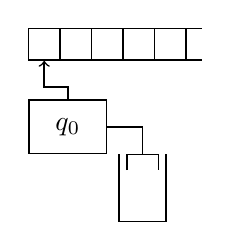
\begin{tikzpicture}

\draw (0.2, 0.2)
  node[draw, line width=0.02cm, , color=black,
       rounded corners=0cm, inner sep=0cm] {

\begin{minipage}[t][0.4cm]{0.4cm}
\mbox{}

\end{minipage}

};\draw (0.2, 0.2) node[color=black] {{\vphantom{\SPACE\SPACE\SPACE\SPACE\SPACE}\texttt{\SPACE}}};
\draw (0.6000000000000001, 0.2)
  node[draw, line width=0.02cm, , color=black,
       rounded corners=0cm, inner sep=0cm] {

\begin{minipage}[t][0.4cm]{0.4cm}
\mbox{}

\end{minipage}

};\draw (0.6000000000000001, 0.2) node[color=black] {{\vphantom{\SPACE\SPACE\SPACE\SPACE\SPACE}\texttt{\SPACE}}};
\draw (1.0, 0.2)
  node[draw, line width=0.02cm, , color=black,
       rounded corners=0cm, inner sep=0cm] {

\begin{minipage}[t][0.4cm]{0.4cm}
\mbox{}

\end{minipage}

};\draw (1.0, 0.2) node[color=black] {{\vphantom{\SPACE\SPACE\SPACE\SPACE\SPACE}\texttt{\SPACE}}};
\draw (1.4000000000000001, 0.2)
  node[draw, line width=0.02cm, , color=black,
       rounded corners=0cm, inner sep=0cm] {

\begin{minipage}[t][0.4cm]{0.4cm}
\mbox{}

\end{minipage}

};\draw (1.4000000000000001, 0.2) node[color=black] {{\vphantom{\SPACE\SPACE\SPACE\SPACE\SPACE}\texttt{\SPACE}}};
\draw (1.7999999999999998, 0.2)
  node[draw, line width=0.02cm, , color=black,
       rounded corners=0cm, inner sep=0cm] {

\begin{minipage}[t][0.4cm]{0.4cm}
\mbox{}

\end{minipage}

};\draw (1.7999999999999998, 0.2) node[color=black] {{\vphantom{\SPACE\SPACE\SPACE\SPACE\SPACE}\texttt{\SPACE}}};\draw[line width=0.02cm,black] (2.0,0.4) to  (2.2,0.4);
\draw[line width=0.02cm,black] (2.0,0.0) to  (2.2,0.0);

\draw (0.5, -0.85)
  node[draw, line width=0.02cm, , color=black,
       rounded corners=0cm, inner sep=0cm] {

\begin{minipage}[t][0.68cm]{0.98cm}
\mbox{}

\end{minipage}

};\draw (0.5, -0.85) node[color=black] {$q_0$};\draw[line width=0.02cm,black,->] (0.5,-0.5) to  (0.5,-0.34) to  (0.2,-0.34) to  (0.2,-0.01);

\draw (1.45, -1.7499999999999998)
  node[draw=none, line width=0cm, , color=black,
       rounded corners=0cm, inner sep=0cm] {

\begin{minipage}[t][0.4cm]{0.4cm}
\mbox{}

\end{minipage}

};\draw[line width=0.02cm,black] (1.15,-1.2) to  (1.15,-2.05) to  (1.75,-2.05) to  (1.75,-1.2);
\draw[line width=0.02cm,black] (1,-0.85) to  (1.45,-0.85) to  (1.45,-1.2);
\draw[line width=0.02cm,black] (1.25,-1.4) to  (1.25,-1.2) to  (1.65,-1.2) to  (1.65,-1.4);
\end{tikzpicture}

\end{center}



Of course this is not a maxheap anymore.
To make this back to a maxheap, clearly the simplest thing to do is
to heapify-down.
In this case I need two swaps.
First I do this swap

\begin{center}
\begin{tikzpicture}

\fill[white] (11.0, 0.0) circle (0.3);
\node [line width=0.03cm,black,minimum size=0.57cm,draw,circle] at (11.0,0.0)(A){};\draw (11.0, 0.0) node[color=black] {\texttt{20}};
\fill[white] (10.0, -0.7) circle (0.3);
\node [line width=0.03cm,black,minimum size=0.57cm,draw,circle] at (10.0,-0.7)(a){};\draw (10.0, -0.7) node[color=black] {\texttt{10}};
\fill[white] (9.0, -1.4) circle (0.3);
\node [line width=0.03cm,black,minimum size=0.57cm,draw,circle] at (9.0,-1.4)(b){};\draw (9.0, -1.4) node[color=black] {\texttt{5}};
\fill[white] (10.0, -2.1) circle (0.3);
\node [line width=0.03cm,black,minimum size=0.57cm,draw,circle] at (10.0,-2.1)(e){};\draw (10.0, -2.1) node[color=black] {\texttt{8}};
\fill[white] (9.0, -2.8) circle (0.3);
\node [line width=0.03cm,black,minimum size=0.57cm,draw,circle] at (9.0,-2.8)(k){};\draw (9.0, -2.8) node[color=black] {\texttt{6}};
\fill[white] (11.0, -2.8) circle (0.3);
\node [line width=0.03cm,black,minimum size=0.57cm,draw,circle] at (11.0,-2.8)(l){};\draw (11.0, -2.8) node[color=black] {\texttt{9}};
\fill[white] (11.0, -1.4) circle (0.3);
\node [line width=0.03cm,black,minimum size=0.57cm,draw,circle] at (11.0,-1.4)(p){};\draw (11.0, -1.4) node[color=black] {\texttt{15}};\draw[line width=0.03cm,black,->,>=triangle 60] (A) to  (a);
\draw[line width=0.03cm,black,->,>=triangle 60] (a) to  (p);
\draw[line width=0.03cm,black,->,>=triangle 60] (a) to  (b);
\draw[line width=0.03cm,black,->,>=triangle 60] (b) to  (e);
\draw[line width=0.03cm,black,->,>=triangle 60] (e) to  (k);
\draw[line width=0.03cm,black,->,>=triangle 60] (e) to  (l);
\end{tikzpicture}

\end{center}



to get this:

\begin{center}
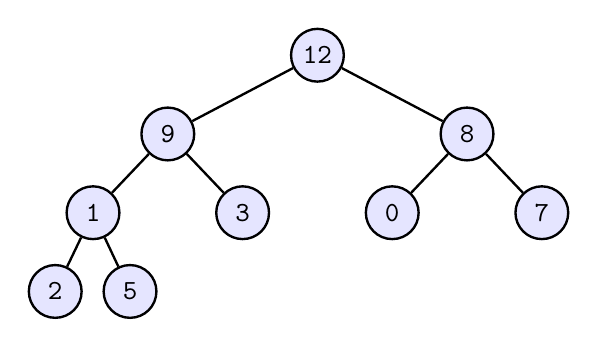
\begin{tikzpicture}

\fill[blue!10] (0.0, 0.0) circle (0.35);
\node [line width=0.03cm,black,minimum size=0.6699999999999999cm,draw,circle] at (0.0,0.0)(12){};\draw (0.0, 0.0) node[color=black] {\texttt{12}};
\fill[blue!10] (-1.9, -1.0) circle (0.35);
\node [line width=0.03cm,black,minimum size=0.6699999999999999cm,draw,circle] at (-1.9,-1.0)(9){};\draw (-1.9, -1.0) node[color=black] {\texttt{9}};
\fill[blue!10] (1.9, -1.0) circle (0.35);
\node [line width=0.03cm,black,minimum size=0.6699999999999999cm,draw,circle] at (1.9,-1.0)(8){};\draw (1.9, -1.0) node[color=black] {\texttt{8}};
\fill[blue!10] (-2.85, -2.0) circle (0.35);
\node [line width=0.03cm,black,minimum size=0.6699999999999999cm,draw,circle] at (-2.85,-2.0)(1){};\draw (-2.85, -2.0) node[color=black] {\texttt{1}};
\fill[blue!10] (-0.95, -2.0) circle (0.35);
\node [line width=0.03cm,black,minimum size=0.6699999999999999cm,draw,circle] at (-0.95,-2.0)(3){};\draw (-0.95, -2.0) node[color=black] {\texttt{3}};
\fill[blue!10] (0.95, -2.0) circle (0.35);
\node [line width=0.03cm,black,minimum size=0.6699999999999999cm,draw,circle] at (0.95,-2.0)(0){};\draw (0.95, -2.0) node[color=black] {\texttt{0}};
\fill[blue!10] (2.85, -2.0) circle (0.35);
\node [line width=0.03cm,black,minimum size=0.6699999999999999cm,draw,circle] at (2.85,-2.0)(7){};\draw (2.85, -2.0) node[color=black] {\texttt{7}};
\fill[blue!10] (-3.33, -3.0) circle (0.35);
\node [line width=0.03cm,black,minimum size=0.6699999999999999cm,draw,circle] at (-3.33,-3.0)(2){};\draw (-3.33, -3.0) node[color=black] {\texttt{2}};
\fill[blue!10] (-2.38, -3.0) circle (0.35);
\node [line width=0.03cm,black,minimum size=0.6699999999999999cm,draw,circle] at (-2.38,-3.0)(5){};\draw (-2.38, -3.0) node[color=black] {\texttt{5}};\draw[line width=0.03cm,black] (12) to  (9);
\draw[line width=0.03cm,black] (12) to  (8);
\draw[line width=0.03cm,black] (9) to  (1);
\draw[line width=0.03cm,black] (9) to  (3);
\draw[line width=0.03cm,black] (8) to  (0);
\draw[line width=0.03cm,black] (8) to  (7);
\draw[line width=0.03cm,black] (1) to  (2);
\draw[line width=0.03cm,black] (1) to  (5);
\end{tikzpicture}

\end{center}



Next I do this swap 

\begin{center}
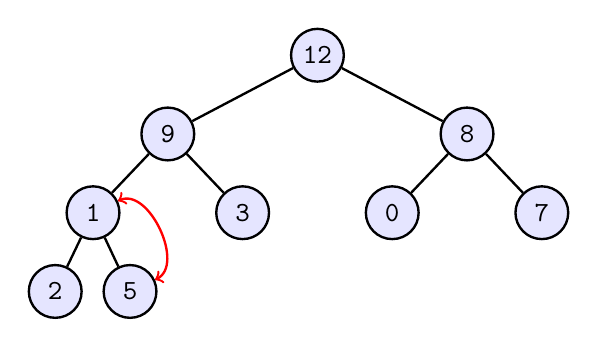
\begin{tikzpicture}

\fill[blue!10] (0.0, 0.0) circle (0.35);
\node [line width=0.03cm,black,minimum size=0.6699999999999999cm,draw,circle] at (0.0,0.0)(12){};\draw (0.0, 0.0) node[color=black] {\texttt{12}};
\fill[blue!10] (-1.9, -1.0) circle (0.35);
\node [line width=0.03cm,black,minimum size=0.6699999999999999cm,draw,circle] at (-1.9,-1.0)(9){};\draw (-1.9, -1.0) node[color=black] {\texttt{9}};
\fill[blue!10] (1.9, -1.0) circle (0.35);
\node [line width=0.03cm,black,minimum size=0.6699999999999999cm,draw,circle] at (1.9,-1.0)(8){};\draw (1.9, -1.0) node[color=black] {\texttt{8}};
\fill[blue!10] (-2.85, -2.0) circle (0.35);
\node [line width=0.03cm,black,minimum size=0.6699999999999999cm,draw,circle] at (-2.85,-2.0)(1){};\draw (-2.85, -2.0) node[color=black] {\texttt{1}};
\fill[blue!10] (-0.95, -2.0) circle (0.35);
\node [line width=0.03cm,black,minimum size=0.6699999999999999cm,draw,circle] at (-0.95,-2.0)(3){};\draw (-0.95, -2.0) node[color=black] {\texttt{3}};
\fill[blue!10] (0.95, -2.0) circle (0.35);
\node [line width=0.03cm,black,minimum size=0.6699999999999999cm,draw,circle] at (0.95,-2.0)(0){};\draw (0.95, -2.0) node[color=black] {\texttt{0}};
\fill[blue!10] (2.85, -2.0) circle (0.35);
\node [line width=0.03cm,black,minimum size=0.6699999999999999cm,draw,circle] at (2.85,-2.0)(7){};\draw (2.85, -2.0) node[color=black] {\texttt{7}};
\fill[blue!10] (-3.33, -3.0) circle (0.35);
\node [line width=0.03cm,black,minimum size=0.6699999999999999cm,draw,circle] at (-3.33,-3.0)(2){};\draw (-3.33, -3.0) node[color=black] {\texttt{2}};
\fill[blue!10] (-2.38, -3.0) circle (0.35);
\node [line width=0.03cm,black,minimum size=0.6699999999999999cm,draw,circle] at (-2.38,-3.0)(5){};\draw (-2.38, -3.0) node[color=black] {\texttt{5}};\draw[line width=0.03cm,black] (12) to  (9);
\draw[line width=0.03cm,black] (12) to  (8);
\draw[line width=0.03cm,black] (9) to  (1);
\draw[line width=0.03cm,black] (9) to  (3);
\draw[line width=0.03cm,black] (8) to  (0);
\draw[line width=0.03cm,black] (8) to  (7);
\draw[line width=0.03cm,black] (1) to  (2);
\draw[line width=0.03cm,black] (1) to  (5);
\draw[line width=0.03cm,red,<->] (1) to [bend left=90]  (5);
\end{tikzpicture}

\end{center}



to get this:

\begin{center}
\begin{tikzpicture}

\fill[white] (20.0, -2.0) circle (0.3);
\node [line width=0.03cm,black,minimum size=0.57cm,draw,circle] at (20.0,-2.0)(A){};\draw (20.0, -2.0) node[color=black] {\texttt{20}};
\fill[white] (14.0, 0.0) circle (0.3);
\node [line width=0.03cm,black,minimum size=0.57cm,draw,circle] at (14.0,0.0)(a){};\draw (14.0, 0.0) node[color=black] {\texttt{10}};
\fill[white] (10.0, -1.0) circle (0.3);
\node [line width=0.03cm,black,minimum size=0.57cm,draw,circle] at (10.0,-1.0)(b){};\draw (10.0, -1.0) node[color=black] {\texttt{4}};
\fill[white] (18.0, -1.0) circle (0.3);
\node [line width=0.03cm,black,minimum size=0.57cm,draw,circle] at (18.0,-1.0)(p){};\draw (18.0, -1.0) node[color=black] {\texttt{18}};
\fill[white] (8.0, -2.0) circle (0.3);
\node [line width=0.03cm,black,minimum size=0.57cm,draw,circle] at (8.0,-2.0)(e){};\draw (8.0, -2.0) node[color=black] {\texttt{2}};
\fill[white] (7.0, -3.0) circle (0.3);
\node [line width=0.03cm,black,minimum size=0.57cm,draw,circle] at (7.0,-3.0)(k){};\draw (7.0, -3.0) node[color=black] {\texttt{0}};
\fill[white] (9.0, -3.0) circle (0.3);
\node [line width=0.03cm,black,minimum size=0.57cm,draw,circle] at (9.0,-3.0)(l){};\draw (9.0, -3.0) node[color=black] {\texttt{3}};
\fill[white] (16.0, -2.0) circle (0.3);
\node [line width=0.03cm,black,minimum size=0.57cm,draw,circle] at (16.0,-2.0)(h){};\draw (16.0, -2.0) node[color=black] {\texttt{15}};
\fill[white] (15.0, -3.0) circle (0.3);
\node [line width=0.03cm,black,minimum size=0.57cm,draw,circle] at (15.0,-3.0)(m){};\draw (15.0, -3.0) node[color=black] {\texttt{12}};
\fill[white] (12.0, -2.0) circle (0.3);
\node [line width=0.03cm,black,minimum size=0.57cm,draw,circle] at (12.0,-2.0)(f){};\draw (12.0, -2.0) node[color=black] {\texttt{8}};
\fill[white] (11.0, -3.0) circle (0.3);
\node [line width=0.03cm,black,minimum size=0.57cm,draw,circle] at (11.0,-3.0)(n){};\draw (11.0, -3.0) node[color=black] {\texttt{6}};
\fill[white] (13.0, -3.0) circle (0.3);
\node [line width=0.03cm,black,minimum size=0.57cm,draw,circle] at (13.0,-3.0)(o){};\draw (13.0, -3.0) node[color=black] {\texttt{9}};
\fill[white] (17.0, -3.0) circle (0.3);
\node [line width=0.03cm,black,minimum size=0.57cm,draw,circle] at (17.0,-3.0)(q){};\draw (17.0, -3.0) node[color=black] {\texttt{17}};
\fill[white] (19.0, -3.0) circle (0.3);
\node [line width=0.03cm,black,minimum size=0.57cm,draw,circle] at (19.0,-3.0)(r){};\draw (19.0, -3.0) node[color=black] {\texttt{19}};
\fill[white] (21.0, -3.0) circle (0.3);
\node [line width=0.03cm,black,minimum size=0.57cm,draw,circle] at (21.0,-3.0)(s){};\draw (21.0, -3.0) node[color=black] {\texttt{22}};\draw[line width=0.03cm,black,->,>=triangle 60] (a) to  (p);
\draw[line width=0.03cm,black,->,>=triangle 60] (h) to  (m);
\draw[line width=0.03cm,black,->,>=triangle 60] (a) to  (b);
\draw[line width=0.03cm,black,->,>=triangle 60] (p) to  (h);
\draw[line width=0.03cm,black,->,>=triangle 60] (p) to  (A);
\draw[line width=0.03cm,black,->,>=triangle 60] (A) to  (r);
\draw[line width=0.03cm,black,->,>=triangle 60] (A) to  (s);
\draw[line width=0.03cm,black,->,>=triangle 60] (b) to  (e);
\draw[line width=0.03cm,black,->,>=triangle 60] (b) to  (f);
\draw[line width=0.03cm,black,->,>=triangle 60] (e) to  (k);
\draw[line width=0.03cm,black,->,>=triangle 60] (e) to  (l);
\draw[line width=0.03cm,black,->,>=triangle 60] (f) to  (o);
\draw[line width=0.03cm,black,->,>=triangle 60] (h) to  (q);
\draw[line width=0.03cm,black,->,>=triangle 60] (f) to  (n);
\end{tikzpicture}

\end{center}



Here's decrease key:

\begin{Verbatim}[frame=single]
ALGORITHM: decrease_key (for maxheap)
INPUT: x - heap (using an array)
       n - length of heap in x
       i - index where key will increase
       k - new key value (k < x[i])

x[i] = k # originally x[i] > k
Perform heapify_down on x at starting at index i.
\end{Verbatim}

The worse runtime of decrease-key for maxheap is clearly
\[
O(\log n)
\]

It's clear that given a heap (max or min), 
you can heapify-up and heapify-down.
I prefer to use 
\lq\lq heapify-up"
and 
\lq\lq heapify-down"
because the important thing is whether a node moves up or down.
In the case of maxheap, 
heapify-up and heapify-down
are respectively
increase-key and decrease-key
whereas
in the case of minheap
heapify-up and heapify-down
are respectively
decrease-key and increase-key.




\newpage
\begin{ex}
Let $x$ be the array
\[
4, 9, 2, 6, 3, 8, 0, 1, 5, 7
\]
First heapify it.
Next do the following:
\begin{tightlist}
  \item Perform increase-key from on the key with value \texttt{2}
  and change it to \texttt{11}.
  \item Perform decrease-key from on the key with value
  \texttt{7} and change it to \texttt{-1}.
\end{tightlist}
\qed
\end{ex}



\newpage
\begin{ex}
Continuing the implementation of the heap ADT using functions,
implement the increase-key and decrease-key
functions:
\begin{console}
int x;
std::vector< int > heap;

heap.resize(5);
heap[0] = 5;
heap[1] = 7;
heap[2] = 8;
heap[3] = 10;
heap[4] = 2;
maxheap_build(heap);      // [10, 7, 8, 5, 2]

maxheap_increasekey(heap, 2, 12); // heap[2] is changed
                          // to 12. heap has to be
                          // reorganized to become
                          // maxheap again.
                          
maxheap_decreasekey(heap, 2, 0); // heap[2] is changed
                          // to 0. heap has to be
                          // reorganized to become
                          // maxheap again.
\end{console}
\end{ex}
